\documentclass[margin=2mm]{standalone}
\usepackage{tikz}
\usepackage{amsmath,amssymb,mathtools}
\begin{document}
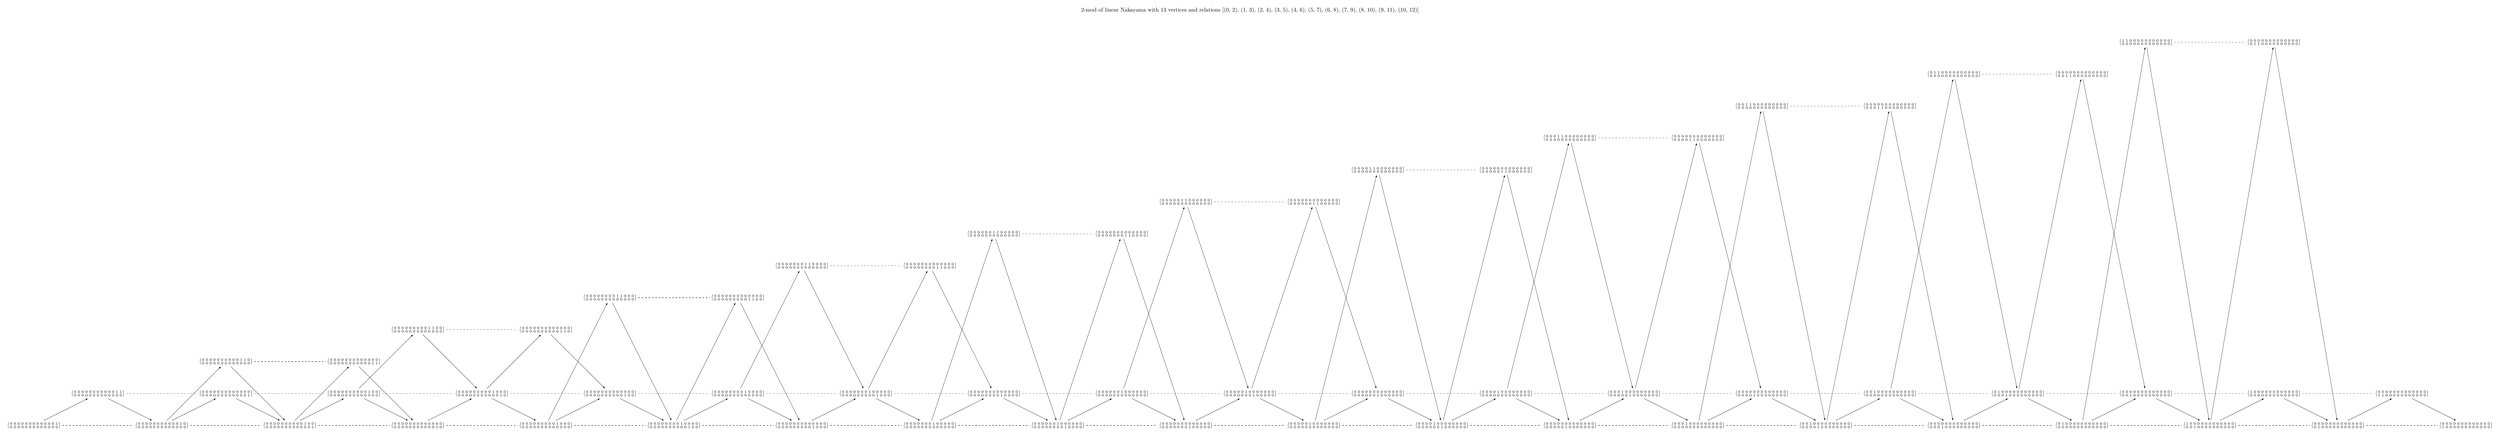
\begin{tikzpicture}[xscale=4,yscale=2]
\node at (19.0,13) [] {$2$-mod of linear Nakayama with 13 vertices and relations [(0, 2), (1, 3), (2, 4), (3, 5), (4, 6), (5, 7), (6, 8), (7, 9), (8, 10), (9, 11), (10, 12)]};
\node (t-0P0) at (33,12) [scale=1] {$\begin{bsmallmatrix}
 1 & 1 & 0 & 0 & 0 & 0 & 0 & 0 & 0 & 0 & 0 & 0 & 0\\
 0 & 0 & 0 & 0 & 0 & 0 & 0 & 0 & 0 & 0 & 0 & 0 & 0\\
\end{bsmallmatrix}$};
\node (t-1P0) at (35,12) [scale=1] {$\begin{bsmallmatrix}
 0 & 0 & 0 & 0 & 0 & 0 & 0 & 0 & 0 & 0 & 0 & 0 & 0\\
 0 & 1 & 1 & 0 & 0 & 0 & 0 & 0 & 0 & 0 & 0 & 0 & 0\\
\end{bsmallmatrix}$};
\node (t-0P1) at (30,11) [scale=1] {$\begin{bsmallmatrix}
 0 & 1 & 1 & 0 & 0 & 0 & 0 & 0 & 0 & 0 & 0 & 0 & 0\\
 0 & 0 & 0 & 0 & 0 & 0 & 0 & 0 & 0 & 0 & 0 & 0 & 0\\
\end{bsmallmatrix}$};
\node (t-1P1) at (32,11) [scale=1] {$\begin{bsmallmatrix}
 0 & 0 & 0 & 0 & 0 & 0 & 0 & 0 & 0 & 0 & 0 & 0 & 0\\
 0 & 0 & 1 & 1 & 0 & 0 & 0 & 0 & 0 & 0 & 0 & 0 & 0\\
\end{bsmallmatrix}$};
\node (t-0P2) at (27,10) [scale=1] {$\begin{bsmallmatrix}
 0 & 0 & 1 & 1 & 0 & 0 & 0 & 0 & 0 & 0 & 0 & 0 & 0\\
 0 & 0 & 0 & 0 & 0 & 0 & 0 & 0 & 0 & 0 & 0 & 0 & 0\\
\end{bsmallmatrix}$};
\node (t-1P2) at (29,10) [scale=1] {$\begin{bsmallmatrix}
 0 & 0 & 0 & 0 & 0 & 0 & 0 & 0 & 0 & 0 & 0 & 0 & 0\\
 0 & 0 & 0 & 1 & 1 & 0 & 0 & 0 & 0 & 0 & 0 & 0 & 0\\
\end{bsmallmatrix}$};
\node (t-0P3) at (24,9) [scale=1] {$\begin{bsmallmatrix}
 0 & 0 & 0 & 1 & 1 & 0 & 0 & 0 & 0 & 0 & 0 & 0 & 0\\
 0 & 0 & 0 & 0 & 0 & 0 & 0 & 0 & 0 & 0 & 0 & 0 & 0\\
\end{bsmallmatrix}$};
\node (t-1P3) at (26,9) [scale=1] {$\begin{bsmallmatrix}
 0 & 0 & 0 & 0 & 0 & 0 & 0 & 0 & 0 & 0 & 0 & 0 & 0\\
 0 & 0 & 0 & 0 & 1 & 1 & 0 & 0 & 0 & 0 & 0 & 0 & 0\\
\end{bsmallmatrix}$};
\node (t-0P4) at (21,8) [scale=1] {$\begin{bsmallmatrix}
 0 & 0 & 0 & 0 & 1 & 1 & 0 & 0 & 0 & 0 & 0 & 0 & 0\\
 0 & 0 & 0 & 0 & 0 & 0 & 0 & 0 & 0 & 0 & 0 & 0 & 0\\
\end{bsmallmatrix}$};
\node (t-1P4) at (23,8) [scale=1] {$\begin{bsmallmatrix}
 0 & 0 & 0 & 0 & 0 & 0 & 0 & 0 & 0 & 0 & 0 & 0 & 0\\
 0 & 0 & 0 & 0 & 0 & 1 & 1 & 0 & 0 & 0 & 0 & 0 & 0\\
\end{bsmallmatrix}$};
\node (t-0P5) at (18,7) [scale=1] {$\begin{bsmallmatrix}
 0 & 0 & 0 & 0 & 0 & 1 & 1 & 0 & 0 & 0 & 0 & 0 & 0\\
 0 & 0 & 0 & 0 & 0 & 0 & 0 & 0 & 0 & 0 & 0 & 0 & 0\\
\end{bsmallmatrix}$};
\node (t-1P5) at (20,7) [scale=1] {$\begin{bsmallmatrix}
 0 & 0 & 0 & 0 & 0 & 0 & 0 & 0 & 0 & 0 & 0 & 0 & 0\\
 0 & 0 & 0 & 0 & 0 & 0 & 1 & 1 & 0 & 0 & 0 & 0 & 0\\
\end{bsmallmatrix}$};
\node (t-0P6) at (15,6) [scale=1] {$\begin{bsmallmatrix}
 0 & 0 & 0 & 0 & 0 & 0 & 1 & 1 & 0 & 0 & 0 & 0 & 0\\
 0 & 0 & 0 & 0 & 0 & 0 & 0 & 0 & 0 & 0 & 0 & 0 & 0\\
\end{bsmallmatrix}$};
\node (t-1P6) at (17,6) [scale=1] {$\begin{bsmallmatrix}
 0 & 0 & 0 & 0 & 0 & 0 & 0 & 0 & 0 & 0 & 0 & 0 & 0\\
 0 & 0 & 0 & 0 & 0 & 0 & 0 & 1 & 1 & 0 & 0 & 0 & 0\\
\end{bsmallmatrix}$};
\node (t-0P7) at (12,5) [scale=1] {$\begin{bsmallmatrix}
 0 & 0 & 0 & 0 & 0 & 0 & 0 & 1 & 1 & 0 & 0 & 0 & 0\\
 0 & 0 & 0 & 0 & 0 & 0 & 0 & 0 & 0 & 0 & 0 & 0 & 0\\
\end{bsmallmatrix}$};
\node (t-1P7) at (14,5) [scale=1] {$\begin{bsmallmatrix}
 0 & 0 & 0 & 0 & 0 & 0 & 0 & 0 & 0 & 0 & 0 & 0 & 0\\
 0 & 0 & 0 & 0 & 0 & 0 & 0 & 0 & 1 & 1 & 0 & 0 & 0\\
\end{bsmallmatrix}$};
\node (t-0P8) at (9,4) [scale=1] {$\begin{bsmallmatrix}
 0 & 0 & 0 & 0 & 0 & 0 & 0 & 0 & 1 & 1 & 0 & 0 & 0\\
 0 & 0 & 0 & 0 & 0 & 0 & 0 & 0 & 0 & 0 & 0 & 0 & 0\\
\end{bsmallmatrix}$};
\node (t-1P8) at (11,4) [scale=1] {$\begin{bsmallmatrix}
 0 & 0 & 0 & 0 & 0 & 0 & 0 & 0 & 0 & 0 & 0 & 0 & 0\\
 0 & 0 & 0 & 0 & 0 & 0 & 0 & 0 & 0 & 1 & 1 & 0 & 0\\
\end{bsmallmatrix}$};
\node (t-0P9) at (6,3) [scale=1] {$\begin{bsmallmatrix}
 0 & 0 & 0 & 0 & 0 & 0 & 0 & 0 & 0 & 1 & 1 & 0 & 0\\
 0 & 0 & 0 & 0 & 0 & 0 & 0 & 0 & 0 & 0 & 0 & 0 & 0\\
\end{bsmallmatrix}$};
\node (t-1P9) at (8,3) [scale=1] {$\begin{bsmallmatrix}
 0 & 0 & 0 & 0 & 0 & 0 & 0 & 0 & 0 & 0 & 0 & 0 & 0\\
 0 & 0 & 0 & 0 & 0 & 0 & 0 & 0 & 0 & 0 & 1 & 1 & 0\\
\end{bsmallmatrix}$};
\node (t-0P10) at (3,2) [scale=1] {$\begin{bsmallmatrix}
 0 & 0 & 0 & 0 & 0 & 0 & 0 & 0 & 0 & 0 & 1 & 1 & 0\\
 0 & 0 & 0 & 0 & 0 & 0 & 0 & 0 & 0 & 0 & 0 & 0 & 0\\
\end{bsmallmatrix}$};
\node (t-1P10) at (5,2) [scale=1] {$\begin{bsmallmatrix}
 0 & 0 & 0 & 0 & 0 & 0 & 0 & 0 & 0 & 0 & 0 & 0 & 0\\
 0 & 0 & 0 & 0 & 0 & 0 & 0 & 0 & 0 & 0 & 0 & 1 & 1\\
\end{bsmallmatrix}$};
\node (t-0P11) at (1,1) [scale=1] {$\begin{bsmallmatrix}
 0 & 0 & 0 & 0 & 0 & 0 & 0 & 0 & 0 & 0 & 0 & 1 & 1\\
 0 & 0 & 0 & 0 & 0 & 0 & 0 & 0 & 0 & 0 & 0 & 0 & 0\\
\end{bsmallmatrix}$};
\node (t-1P11) at (3,1) [scale=1] {$\begin{bsmallmatrix}
 0 & 0 & 0 & 0 & 0 & 0 & 0 & 0 & 0 & 0 & 0 & 0 & 0\\
 0 & 0 & 0 & 0 & 0 & 0 & 0 & 0 & 0 & 0 & 0 & 0 & 1\\
\end{bsmallmatrix}$};
\node (t-2P11) at (5,1) [scale=1] {$\begin{bsmallmatrix}
 0 & 0 & 0 & 0 & 0 & 0 & 0 & 0 & 0 & 0 & 1 & 0 & 0\\
 0 & 0 & 0 & 0 & 0 & 0 & 0 & 0 & 0 & 0 & 0 & 0 & 0\\
\end{bsmallmatrix}$};
\node (t-3P11) at (7,1) [scale=1] {$\begin{bsmallmatrix}
 0 & 0 & 0 & 0 & 0 & 0 & 0 & 0 & 0 & 1 & 0 & 0 & 0\\
 0 & 0 & 0 & 0 & 0 & 0 & 0 & 0 & 0 & 0 & 0 & 1 & 0\\
\end{bsmallmatrix}$};
\node (t-4P11) at (9,1) [scale=1] {$\begin{bsmallmatrix}
 0 & 0 & 0 & 0 & 0 & 0 & 0 & 0 & 0 & 0 & 0 & 0 & 0\\
 0 & 0 & 0 & 0 & 0 & 0 & 0 & 0 & 0 & 0 & 1 & 0 & 0\\
\end{bsmallmatrix}$};
\node (t-5P11) at (11,1) [scale=1] {$\begin{bsmallmatrix}
 0 & 0 & 0 & 0 & 0 & 0 & 0 & 0 & 1 & 0 & 0 & 0 & 0\\
 0 & 0 & 0 & 0 & 0 & 0 & 0 & 0 & 0 & 0 & 0 & 0 & 0\\
\end{bsmallmatrix}$};
\node (t-6P11) at (13,1) [scale=1] {$\begin{bsmallmatrix}
 0 & 0 & 0 & 0 & 0 & 0 & 0 & 1 & 0 & 0 & 0 & 0 & 0\\
 0 & 0 & 0 & 0 & 0 & 0 & 0 & 0 & 0 & 1 & 0 & 0 & 0\\
\end{bsmallmatrix}$};
\node (t-7P11) at (15,1) [scale=1] {$\begin{bsmallmatrix}
 0 & 0 & 0 & 0 & 0 & 0 & 0 & 0 & 0 & 0 & 0 & 0 & 0\\
 0 & 0 & 0 & 0 & 0 & 0 & 0 & 0 & 1 & 0 & 0 & 0 & 0\\
\end{bsmallmatrix}$};
\node (t-8P11) at (17,1) [scale=1] {$\begin{bsmallmatrix}
 0 & 0 & 0 & 0 & 0 & 0 & 1 & 0 & 0 & 0 & 0 & 0 & 0\\
 0 & 0 & 0 & 0 & 0 & 0 & 0 & 0 & 0 & 0 & 0 & 0 & 0\\
\end{bsmallmatrix}$};
\node (t-9P11) at (19,1) [scale=1] {$\begin{bsmallmatrix}
 0 & 0 & 0 & 0 & 0 & 1 & 0 & 0 & 0 & 0 & 0 & 0 & 0\\
 0 & 0 & 0 & 0 & 0 & 0 & 0 & 1 & 0 & 0 & 0 & 0 & 0\\
\end{bsmallmatrix}$};
\node (t-10P11) at (21,1) [scale=1] {$\begin{bsmallmatrix}
 0 & 0 & 0 & 0 & 0 & 0 & 0 & 0 & 0 & 0 & 0 & 0 & 0\\
 0 & 0 & 0 & 0 & 0 & 0 & 1 & 0 & 0 & 0 & 0 & 0 & 0\\
\end{bsmallmatrix}$};
\node (t-11P11) at (23,1) [scale=1] {$\begin{bsmallmatrix}
 0 & 0 & 0 & 0 & 1 & 0 & 0 & 0 & 0 & 0 & 0 & 0 & 0\\
 0 & 0 & 0 & 0 & 0 & 0 & 0 & 0 & 0 & 0 & 0 & 0 & 0\\
\end{bsmallmatrix}$};
\node (t-12P11) at (25,1) [scale=1] {$\begin{bsmallmatrix}
 0 & 0 & 0 & 1 & 0 & 0 & 0 & 0 & 0 & 0 & 0 & 0 & 0\\
 0 & 0 & 0 & 0 & 0 & 1 & 0 & 0 & 0 & 0 & 0 & 0 & 0\\
\end{bsmallmatrix}$};
\node (t-13P11) at (27,1) [scale=1] {$\begin{bsmallmatrix}
 0 & 0 & 0 & 0 & 0 & 0 & 0 & 0 & 0 & 0 & 0 & 0 & 0\\
 0 & 0 & 0 & 0 & 1 & 0 & 0 & 0 & 0 & 0 & 0 & 0 & 0\\
\end{bsmallmatrix}$};
\node (t-14P11) at (29,1) [scale=1] {$\begin{bsmallmatrix}
 0 & 0 & 1 & 0 & 0 & 0 & 0 & 0 & 0 & 0 & 0 & 0 & 0\\
 0 & 0 & 0 & 0 & 0 & 0 & 0 & 0 & 0 & 0 & 0 & 0 & 0\\
\end{bsmallmatrix}$};
\node (t-15P11) at (31,1) [scale=1] {$\begin{bsmallmatrix}
 0 & 1 & 0 & 0 & 0 & 0 & 0 & 0 & 0 & 0 & 0 & 0 & 0\\
 0 & 0 & 0 & 1 & 0 & 0 & 0 & 0 & 0 & 0 & 0 & 0 & 0\\
\end{bsmallmatrix}$};
\node (t-16P11) at (33,1) [scale=1] {$\begin{bsmallmatrix}
 0 & 0 & 0 & 0 & 0 & 0 & 0 & 0 & 0 & 0 & 0 & 0 & 0\\
 0 & 0 & 1 & 0 & 0 & 0 & 0 & 0 & 0 & 0 & 0 & 0 & 0\\
\end{bsmallmatrix}$};
\node (t-17P11) at (35,1) [scale=1] {$\begin{bsmallmatrix}
 1 & 0 & 0 & 0 & 0 & 0 & 0 & 0 & 0 & 0 & 0 & 0 & 0\\
 0 & 0 & 0 & 0 & 0 & 0 & 0 & 0 & 0 & 0 & 0 & 0 & 0\\
\end{bsmallmatrix}$};
\node (t-18P11) at (37,1) [scale=1] {$\begin{bsmallmatrix}
 0 & 0 & 0 & 0 & 0 & 0 & 0 & 0 & 0 & 0 & 0 & 0 & 0\\
 1 & 1 & 0 & 0 & 0 & 0 & 0 & 0 & 0 & 0 & 0 & 0 & 0\\
\end{bsmallmatrix}$};
\node (t-0P12) at (0,0) [scale=1] {$\begin{bsmallmatrix}
 0 & 0 & 0 & 0 & 0 & 0 & 0 & 0 & 0 & 0 & 0 & 0 & 1\\
 0 & 0 & 0 & 0 & 0 & 0 & 0 & 0 & 0 & 0 & 0 & 0 & 0\\
\end{bsmallmatrix}$};
\node (t-1P12) at (2,0) [scale=1] {$\begin{bsmallmatrix}
 0 & 0 & 0 & 0 & 0 & 0 & 0 & 0 & 0 & 0 & 0 & 1 & 0\\
 0 & 0 & 0 & 0 & 0 & 0 & 0 & 0 & 0 & 0 & 0 & 0 & 0\\
\end{bsmallmatrix}$};
\node (t-2P12) at (4,0) [scale=1] {$\begin{bsmallmatrix}
 0 & 0 & 0 & 0 & 0 & 0 & 0 & 0 & 0 & 0 & 1 & 0 & 0\\
 0 & 0 & 0 & 0 & 0 & 0 & 0 & 0 & 0 & 0 & 0 & 0 & 1\\
\end{bsmallmatrix}$};
\node (t-3P12) at (6,0) [scale=1] {$\begin{bsmallmatrix}
 0 & 0 & 0 & 0 & 0 & 0 & 0 & 0 & 0 & 0 & 0 & 0 & 0\\
 0 & 0 & 0 & 0 & 0 & 0 & 0 & 0 & 0 & 0 & 0 & 1 & 0\\
\end{bsmallmatrix}$};
\node (t-4P12) at (8,0) [scale=1] {$\begin{bsmallmatrix}
 0 & 0 & 0 & 0 & 0 & 0 & 0 & 0 & 0 & 1 & 0 & 0 & 0\\
 0 & 0 & 0 & 0 & 0 & 0 & 0 & 0 & 0 & 0 & 0 & 0 & 0\\
\end{bsmallmatrix}$};
\node (t-5P12) at (10,0) [scale=1] {$\begin{bsmallmatrix}
 0 & 0 & 0 & 0 & 0 & 0 & 0 & 0 & 1 & 0 & 0 & 0 & 0\\
 0 & 0 & 0 & 0 & 0 & 0 & 0 & 0 & 0 & 0 & 1 & 0 & 0\\
\end{bsmallmatrix}$};
\node (t-6P12) at (12,0) [scale=1] {$\begin{bsmallmatrix}
 0 & 0 & 0 & 0 & 0 & 0 & 0 & 0 & 0 & 0 & 0 & 0 & 0\\
 0 & 0 & 0 & 0 & 0 & 0 & 0 & 0 & 0 & 1 & 0 & 0 & 0\\
\end{bsmallmatrix}$};
\node (t-7P12) at (14,0) [scale=1] {$\begin{bsmallmatrix}
 0 & 0 & 0 & 0 & 0 & 0 & 0 & 1 & 0 & 0 & 0 & 0 & 0\\
 0 & 0 & 0 & 0 & 0 & 0 & 0 & 0 & 0 & 0 & 0 & 0 & 0\\
\end{bsmallmatrix}$};
\node (t-8P12) at (16,0) [scale=1] {$\begin{bsmallmatrix}
 0 & 0 & 0 & 0 & 0 & 0 & 1 & 0 & 0 & 0 & 0 & 0 & 0\\
 0 & 0 & 0 & 0 & 0 & 0 & 0 & 0 & 1 & 0 & 0 & 0 & 0\\
\end{bsmallmatrix}$};
\node (t-9P12) at (18,0) [scale=1] {$\begin{bsmallmatrix}
 0 & 0 & 0 & 0 & 0 & 0 & 0 & 0 & 0 & 0 & 0 & 0 & 0\\
 0 & 0 & 0 & 0 & 0 & 0 & 0 & 1 & 0 & 0 & 0 & 0 & 0\\
\end{bsmallmatrix}$};
\node (t-10P12) at (20,0) [scale=1] {$\begin{bsmallmatrix}
 0 & 0 & 0 & 0 & 0 & 1 & 0 & 0 & 0 & 0 & 0 & 0 & 0\\
 0 & 0 & 0 & 0 & 0 & 0 & 0 & 0 & 0 & 0 & 0 & 0 & 0\\
\end{bsmallmatrix}$};
\node (t-11P12) at (22,0) [scale=1] {$\begin{bsmallmatrix}
 0 & 0 & 0 & 0 & 1 & 0 & 0 & 0 & 0 & 0 & 0 & 0 & 0\\
 0 & 0 & 0 & 0 & 0 & 0 & 1 & 0 & 0 & 0 & 0 & 0 & 0\\
\end{bsmallmatrix}$};
\node (t-12P12) at (24,0) [scale=1] {$\begin{bsmallmatrix}
 0 & 0 & 0 & 0 & 0 & 0 & 0 & 0 & 0 & 0 & 0 & 0 & 0\\
 0 & 0 & 0 & 0 & 0 & 1 & 0 & 0 & 0 & 0 & 0 & 0 & 0\\
\end{bsmallmatrix}$};
\node (t-13P12) at (26,0) [scale=1] {$\begin{bsmallmatrix}
 0 & 0 & 0 & 1 & 0 & 0 & 0 & 0 & 0 & 0 & 0 & 0 & 0\\
 0 & 0 & 0 & 0 & 0 & 0 & 0 & 0 & 0 & 0 & 0 & 0 & 0\\
\end{bsmallmatrix}$};
\node (t-14P12) at (28,0) [scale=1] {$\begin{bsmallmatrix}
 0 & 0 & 1 & 0 & 0 & 0 & 0 & 0 & 0 & 0 & 0 & 0 & 0\\
 0 & 0 & 0 & 0 & 1 & 0 & 0 & 0 & 0 & 0 & 0 & 0 & 0\\
\end{bsmallmatrix}$};
\node (t-15P12) at (30,0) [scale=1] {$\begin{bsmallmatrix}
 0 & 0 & 0 & 0 & 0 & 0 & 0 & 0 & 0 & 0 & 0 & 0 & 0\\
 0 & 0 & 0 & 1 & 0 & 0 & 0 & 0 & 0 & 0 & 0 & 0 & 0\\
\end{bsmallmatrix}$};
\node (t-16P12) at (32,0) [scale=1] {$\begin{bsmallmatrix}
 0 & 1 & 0 & 0 & 0 & 0 & 0 & 0 & 0 & 0 & 0 & 0 & 0\\
 0 & 0 & 0 & 0 & 0 & 0 & 0 & 0 & 0 & 0 & 0 & 0 & 0\\
\end{bsmallmatrix}$};
\node (t-17P12) at (34,0) [scale=1] {$\begin{bsmallmatrix}
 1 & 0 & 0 & 0 & 0 & 0 & 0 & 0 & 0 & 0 & 0 & 0 & 0\\
 0 & 0 & 1 & 0 & 0 & 0 & 0 & 0 & 0 & 0 & 0 & 0 & 0\\
\end{bsmallmatrix}$};
\node (t-18P12) at (36,0) [scale=1] {$\begin{bsmallmatrix}
 0 & 0 & 0 & 0 & 0 & 0 & 0 & 0 & 0 & 0 & 0 & 0 & 0\\
 0 & 1 & 0 & 0 & 0 & 0 & 0 & 0 & 0 & 0 & 0 & 0 & 0\\
\end{bsmallmatrix}$};
\node (t-19P12) at (38,0) [scale=1] {$\begin{bsmallmatrix}
 0 & 0 & 0 & 0 & 0 & 0 & 0 & 0 & 0 & 0 & 0 & 0 & 0\\
 1 & 0 & 0 & 0 & 0 & 0 & 0 & 0 & 0 & 0 & 0 & 0 & 0\\
\end{bsmallmatrix}$};
\draw[-latex] (t-0P0) -- (t-17P12);
\draw[-latex] (t-1P0) -- (t-18P12);
\draw[-latex] (t-0P1) -- (t-15P11);
\draw[-latex] (t-1P1) -- (t-16P11);
\draw[-latex] (t-0P2) -- (t-14P12);
\draw[-latex] (t-1P2) -- (t-15P12);
\draw[-latex] (t-0P3) -- (t-12P11);
\draw[-latex] (t-1P3) -- (t-13P11);
\draw[-latex] (t-0P4) -- (t-11P12);
\draw[-latex] (t-1P4) -- (t-12P12);
\draw[-latex] (t-0P5) -- (t-9P11);
\draw[-latex] (t-1P5) -- (t-10P11);
\draw[-latex] (t-0P6) -- (t-8P12);
\draw[-latex] (t-1P6) -- (t-9P12);
\draw[-latex] (t-0P7) -- (t-6P11);
\draw[-latex] (t-1P7) -- (t-7P11);
\draw[-latex] (t-0P8) -- (t-5P12);
\draw[-latex] (t-1P8) -- (t-6P12);
\draw[-latex] (t-0P9) -- (t-3P11);
\draw[-latex] (t-1P9) -- (t-4P11);
\draw[-latex] (t-0P10) -- (t-2P12);
\draw[-latex] (t-1P10) -- (t-3P12);
\draw[-latex] (t-0P11) -- (t-1P12);
\draw[-latex] (t-1P11) -- (t-2P12);
\draw[-latex] (t-2P11) -- (t-0P9);
\draw[-latex] (t-2P11) -- (t-3P12);
\draw[-latex] (t-3P11) -- (t-4P12);
\draw[-latex] (t-3P11) -- (t-1P9);
\draw[-latex] (t-4P11) -- (t-5P12);
\draw[-latex] (t-5P11) -- (t-0P7);
\draw[-latex] (t-5P11) -- (t-6P12);
\draw[-latex] (t-6P11) -- (t-7P12);
\draw[-latex] (t-6P11) -- (t-1P7);
\draw[-latex] (t-7P11) -- (t-8P12);
\draw[-latex] (t-8P11) -- (t-0P5);
\draw[-latex] (t-8P11) -- (t-9P12);
\draw[-latex] (t-9P11) -- (t-10P12);
\draw[-latex] (t-9P11) -- (t-1P5);
\draw[-latex] (t-10P11) -- (t-11P12);
\draw[-latex] (t-11P11) -- (t-0P3);
\draw[-latex] (t-11P11) -- (t-12P12);
\draw[-latex] (t-12P11) -- (t-13P12);
\draw[-latex] (t-12P11) -- (t-1P3);
\draw[-latex] (t-13P11) -- (t-14P12);
\draw[-latex] (t-14P11) -- (t-0P1);
\draw[-latex] (t-14P11) -- (t-15P12);
\draw[-latex] (t-15P11) -- (t-16P12);
\draw[-latex] (t-15P11) -- (t-1P1);
\draw[-latex] (t-16P11) -- (t-17P12);
\draw[-latex] (t-17P11) -- (t-18P12);
\draw[-latex] (t-18P11) -- (t-19P12);
\draw[-latex] (t-0P12) -- (t-0P11);
\draw[-latex] (t-1P12) -- (t-0P10);
\draw[-latex] (t-1P12) -- (t-1P11);
\draw[-latex] (t-2P12) -- (t-1P10);
\draw[-latex] (t-2P12) -- (t-2P11);
\draw[-latex] (t-3P12) -- (t-3P11);
\draw[-latex] (t-4P12) -- (t-0P8);
\draw[-latex] (t-4P12) -- (t-4P11);
\draw[-latex] (t-5P12) -- (t-1P8);
\draw[-latex] (t-5P12) -- (t-5P11);
\draw[-latex] (t-6P12) -- (t-6P11);
\draw[-latex] (t-7P12) -- (t-0P6);
\draw[-latex] (t-7P12) -- (t-7P11);
\draw[-latex] (t-8P12) -- (t-1P6);
\draw[-latex] (t-8P12) -- (t-8P11);
\draw[-latex] (t-9P12) -- (t-9P11);
\draw[-latex] (t-10P12) -- (t-0P4);
\draw[-latex] (t-10P12) -- (t-10P11);
\draw[-latex] (t-11P12) -- (t-1P4);
\draw[-latex] (t-11P12) -- (t-11P11);
\draw[-latex] (t-12P12) -- (t-12P11);
\draw[-latex] (t-13P12) -- (t-0P2);
\draw[-latex] (t-13P12) -- (t-13P11);
\draw[-latex] (t-14P12) -- (t-1P2);
\draw[-latex] (t-14P12) -- (t-14P11);
\draw[-latex] (t-15P12) -- (t-15P11);
\draw[-latex] (t-16P12) -- (t-0P0);
\draw[-latex] (t-16P12) -- (t-16P11);
\draw[-latex] (t-17P12) -- (t-1P0);
\draw[-latex] (t-17P12) -- (t-17P11);
\draw[-latex] (t-18P12) -- (t-18P11);
\draw[dashed] (t-0P0)--(t-1P0);
\draw[dashed] (t-0P1)--(t-1P1);
\draw[dashed] (t-0P2)--(t-1P2);
\draw[dashed] (t-0P3)--(t-1P3);
\draw[dashed] (t-0P4)--(t-1P4);
\draw[dashed] (t-0P5)--(t-1P5);
\draw[dashed] (t-0P6)--(t-1P6);
\draw[dashed] (t-0P7)--(t-1P7);
\draw[dashed] (t-0P8)--(t-1P8);
\draw[dashed] (t-0P9)--(t-1P9);
\draw[dashed] (t-0P10)--(t-1P10);
\draw[dashed] (t-0P11)--(t-1P11);
\draw[dashed] (t-1P11)--(t-2P11);
\draw[dashed] (t-2P11)--(t-3P11);
\draw[dashed] (t-3P11)--(t-4P11);
\draw[dashed] (t-4P11)--(t-5P11);
\draw[dashed] (t-5P11)--(t-6P11);
\draw[dashed] (t-6P11)--(t-7P11);
\draw[dashed] (t-7P11)--(t-8P11);
\draw[dashed] (t-8P11)--(t-9P11);
\draw[dashed] (t-9P11)--(t-10P11);
\draw[dashed] (t-10P11)--(t-11P11);
\draw[dashed] (t-11P11)--(t-12P11);
\draw[dashed] (t-12P11)--(t-13P11);
\draw[dashed] (t-13P11)--(t-14P11);
\draw[dashed] (t-14P11)--(t-15P11);
\draw[dashed] (t-15P11)--(t-16P11);
\draw[dashed] (t-16P11)--(t-17P11);
\draw[dashed] (t-17P11)--(t-18P11);
\draw[dashed] (t-0P12)--(t-1P12);
\draw[dashed] (t-1P12)--(t-2P12);
\draw[dashed] (t-2P12)--(t-3P12);
\draw[dashed] (t-3P12)--(t-4P12);
\draw[dashed] (t-4P12)--(t-5P12);
\draw[dashed] (t-5P12)--(t-6P12);
\draw[dashed] (t-6P12)--(t-7P12);
\draw[dashed] (t-7P12)--(t-8P12);
\draw[dashed] (t-8P12)--(t-9P12);
\draw[dashed] (t-9P12)--(t-10P12);
\draw[dashed] (t-10P12)--(t-11P12);
\draw[dashed] (t-11P12)--(t-12P12);
\draw[dashed] (t-12P12)--(t-13P12);
\draw[dashed] (t-13P12)--(t-14P12);
\draw[dashed] (t-14P12)--(t-15P12);
\draw[dashed] (t-15P12)--(t-16P12);
\draw[dashed] (t-16P12)--(t-17P12);
\draw[dashed] (t-17P12)--(t-18P12);
\draw[dashed] (t-18P12)--(t-19P12);
\end{tikzpicture}\end{document}